\section{Tiles and Tribulations}

You're given a grid of size $n \times n$, where $n = 2^k$ for some $k \ge 1$, with one cell missing. Your job is to cover the board with \textit{L-tiles}. An L-tile is three squares that form an L shape (i.e., a $2\times 2$ square with one square missing). Below is a $4 \times 4$ board, with a missing cell at position $(2,3)$ (using 1-based indexing from bottom left).

\begin{figure}[tbh!]
	\centering
	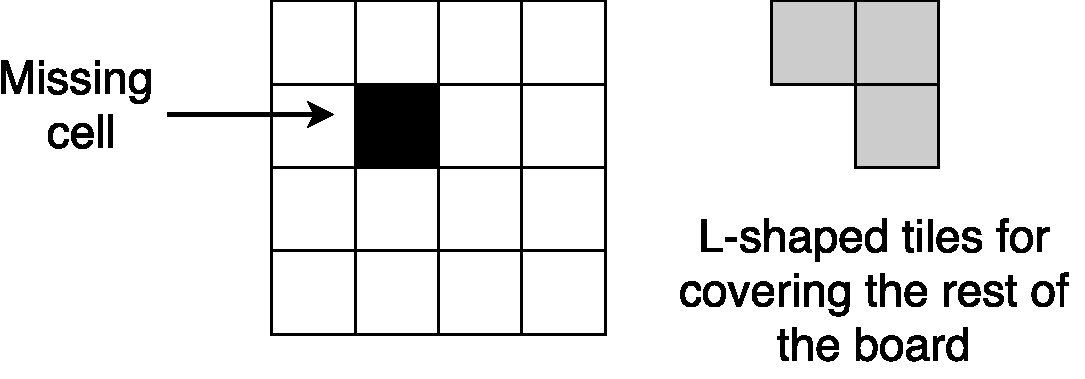
\includegraphics[width=0.6\columnwidth]{a4-tiles.pdf}
\end{figure}

The L-tiles:
\begin{itemize}
	\item Must cover every white square of the board.
	\item Must NOT cover the single black square on the board.
	\item Are not allowed to overlap.
\end{itemize}

\begin{questions}
	\question[5] Prove that, for any $2^k \times 2^k$ board with an arbitrary missing cell, we can come up with a way to cover the board with L-tiles. (Hint: induction on $k$ works well.)

	\begin{soln}
		For a \(2^1 \times 2^1\) board we can cover the board using one \(L-tile\) by removing any arbitrary square, thus our base case \(n = 1\) holds.

		Assume that we can cover any \(2^k \times 2^k\) board using \(L\)-tiles when a square is missing with \(k \geq 1\).

		Now consider a \(2^{k+1} \times 2^{k+1}\) board with an arbitrary missing square.

		We partition this \(2^{k+1} \times 2^{k+1}\) board into four \(2^k \times 2^k\) quadrants, each of which maintains the structure of a square. We label them \(Q_1, Q_2, Q_3, Q_4\) using traditional convention that \(Q_1\) is top-right quadrant and so forth.

		The removed cell must appear in at least one of these sections. By the inductive hypothesis, we can cover it using \(L-tiles\).

		WLOG, assume the missing cell is in top-right quadrant, \(Q_1\). If not, we can rotate our board and relabel the quadrants accordingly.

		Then observe that the bottom-right square of \(Q_2\), the top-right square of \(Q_3\), and the top-left square of \(Q_4\) forms an \(L-tile\).

		Remove these cells from the respective quadrants and we get that by the inductive hypothesis we can cover those qudrants using \(L-tiles\).

		Return the cells using the described \(L-tile\) and we get that we can cover the \(2^{k+1} \times 2^{k+1}\) board using \(L-tiles\) with a square missing.

	\end{soln}


	\ifsolutions\input{q1a-sol.tex}\fi

	\question[5] Design a divide-and-conquer algorithm to place L-tiles to cover a $2^k \times 2^k$ board with a single missing cell.

		\begin{soln}
     \(B\) can be thought of as an \( n \times n \) matrix where \( n = 2^k \) for some integer \( k \geq 1 \). The matrix represents a square board. 

      For ease of notation we may also say \(B = \{(i, j) : 1 \leq i, j \leq n\}\).

      The coordinate \((1, 1)\) refers to the bottom-left corner of the board, in particualar it's the origin.

      For \((i, j)\), first coordinate denotes horizontal position, second coordinate denotes vertical position.

      The solution \( S \) is defined as a collection of sets of coordinates \( \{L_1, L_2, \dots, L_m\} \), where each \( L_i \) is a set of three coordinates that together form an \( L \)-shape.

      We say that \(L_i\) is an \(L-shape\) if each of its coordinates are adjacent to each other and they do not form a \(3-cell\) line.

      Additionally, the sets must satisfy the following conditions, where \((x, y)\) is the missing cell:
    \[
      \bigcap_{i=1}^{m} L_i = \varnothing \quad \text{(pairwise disjoint)}, \quad \text{and} \quad \bigcup_{i=1}^{m} L_i = B \setminus \{(x, y)\} \quad \text{(fully covers the board)}.
    \]

			\begin{algorithmic}[1]
        \Procedure{Cover-Board}{$B$, $n$, $(x, y)$}
        \If {$n = 2$}
        \State \Return {$B \setminus \{(x, y)\}$}
        \EndIf
        \State $B_1 \gets \text{First Qaudrant of } B$ 
        \State $B_2 \gets \text{Second Qaudrant of } B$ 
        \State $B_3 \gets \text{Third Qaudrant of } B$ 
        \State $B_4 \gets \text{Fourth Qaudrant of } B$ 

        \State $L \gets$ Middle square coordinates

        \State Identify $l \in \{1, 2, 3, 4\}$ such that {$(x, y) \in B_l$}
        \State $L := L \setminus B_l$

        \State $L' \gets L \cup \{(x, y)\}$

        \State $B_1 = \text{Cover-Board($B_1$, $\frac{n}{2}$, $B_1 \cap L$)} $
        \State $B_2 = \text{Cover-Board($B_2$, $\frac{n}{2}$, $B_2 \cap L$)} $
        \State $B_3 = \text{Cover-Board($B_3$, $\frac{n}{2}$, $B_3 \cap L$)} $
        \State $B_4 = \text{Cover-Board($B_4$, $\frac{n}{2}$, $B_4 \cap L$)} $
        \State \Return $B_1 \cup B_2 \cup B_3 \cup B_4 \cup L$
				\EndProcedure
			\end{algorithmic}

			\begin{algorithmic}[1]
				\Procedure{Wrapper-Call}{$B$, $n$, $(x, y)$}
        \State \Return \text{Cover-Board}($B$, $n$, $(x, y)$)
				\EndProcedure
			\end{algorithmic}

	\end{soln}

	\ifsolutions\input{q1b-sol.tex}\fi

	\question[2] Give and briefly justify a good asymptotic bound on the runtime of your algorithm in terms of $n$ (the dimension of the board).

  \begin{soln}
    We can model this using a recurrence relation.

    We see that \(T(2) = O(1)\), since we are just returning a set without a particular element.

    Then to create each of \(B_1, B_2, B_3, B_4\) this will take \(O(n^2)\) time since we have to iterate through the entire oringal matrix to create them.

    Determining the set \(L\) will take \(O(1)\) time because we can query it using the passed in parameter \(n\).

    Each of the recursive calls will take \(T(\frac{n}{2})\) time, and the return statement takes \(O(\frac{n^2}{3})\) because we are supposed to merge together sets of size \(3\), which form partitions of \(B\). 

    But we have \(\frac{n^2 - 1}{3}\) of those sets.

    Thus, we can model this with 

   \[
T(n) = \begin{cases} 
      4T\left(\frac{n}{2}\right) + O(n^2), & n > 2 \\
      O(1), & n = 2
    \end{cases}
\]

    We see that \(n^2 \in \Theta (n^{\log_2(4)}\log^0(n))\), thus the master theorem says \(T(n) \in \Theta(n^2 \log(n))\).



  
  \end{soln}

	\ifsolutions\input{q1c-sol.tex}\fi

\end{questions}

